\chapter{State of the Art}
\label{state_of_the_art}

In this chapter, the current state of the art regarding garment folding is presented. Different approaches when working with garments can be found in the literature, and they will be described in this chapter.

Some approaches use 3D computer vision algorithms to create models of the garments or to fit captured gament data to a predefined model. These garment models are used then to apply folding algorithms or to select the best points for manipulation. Some of these models are borrowed from the Computer Graphics community, where garment representation and simulation has been widely studied to achieve realistic clothes behavior in Computer Graphics scenes. This will be covered in section \ref{sota:garment_model_based}.

In other approaches, the problem of garment folding is solved through robot interaction with the garment. By regrasping and changing the garment configuration, the garment category and current pose is detected, and the garment can be led to a target pose. These approaches will be seen in section \ref{sota:garment_manipulation_based}.

Finally, the european project CloPeMa (Clothes Perception and Manipulation), devoted to perception and manipulation of fabric, textiles and garments, is described. Their research most relevant to this thesis is explained in the last section \ref{sota:clopema}.

\section{Garment Modeling-Based Approaches}
\label{sota:garment_model_based}
A significant amount of work conducted in this topic has been focused on modeling the different garment categories for both unfolded, extended garments and for grasped garments. The computer graphics community has also contributed with extensive work on the specifics of clothes modeling due to their need for realistic representation of fabrics and garments. A review of these modeling methods can be found in \cite{Chen2009}. 

Kita et al. propose a method that uses a deformable model to calculate the state of hanging clothes based on 3D observed data \cite{Kita2004, Kita2009}. This calculation is performed by generating a set of candidate shapes predicted by physical simulations of hanging clothes and later comparison of them with the observed data. To fit the observed 3D data better, each generated shape is further deformed and the shape that is more consistent with the observed data is selected. 

\begin{figure}[thpb]
    \centering
    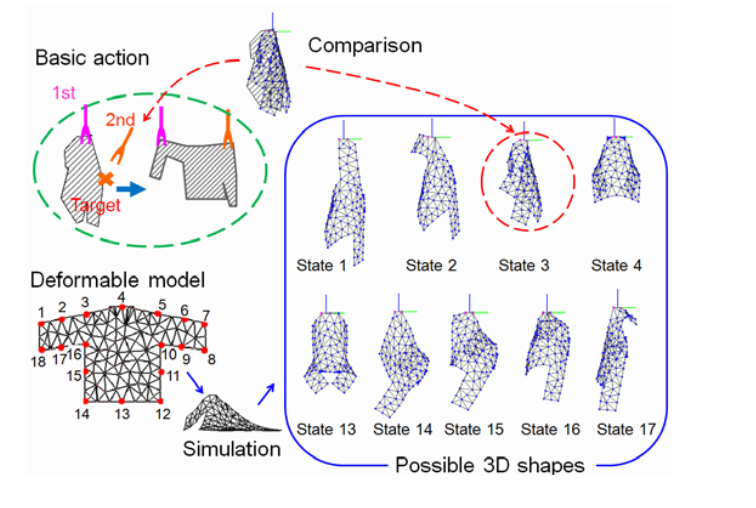
\includegraphics[width=0.95
    \textwidth]{figures/SOTA_Kita_2009.png}
    \caption[dummy]{Basic action and model-driven strategy presented by Kita \cite{Kita2009} \comment{(?)}. The garment is held by a point with a robotic arm and different deformable models are tested against the garment data. The model that explains the best the data is selected to calculate the second grasping point. }
    \label{fig:SOTA_Kita_2009}
\end{figure}

Miller et al. present an approach to modeling the clothes when already spread out on a flat surface in \cite{Miller2011}. A series of parametrized shape models are proposed, each clothing category having its own model. Garment variability is solved through variation of those parameters. Once the garment has been modeled with their method, a preprogrammed folding sequence can be performed.

%\begin{figure}[thpb]
%    \centering
%    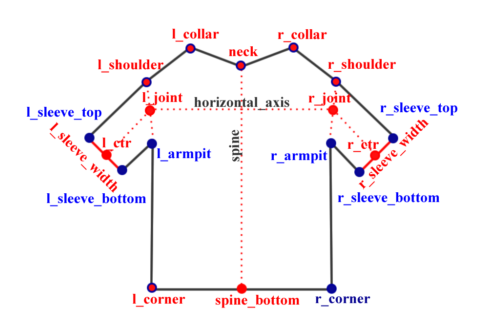
\includegraphics[width=0.6
%    \textwidth]{figures/SOTA_Miller_2011.png}
%    \caption{\comment{(Miller thing - add more models)}}
%    \label{fig:SOTA_Miller_2011}
%\end{figure}

\begin{figure}[htbp]
	\centering
    \begin{subfigure}[l]{0.49\textwidth}
        \centering
    	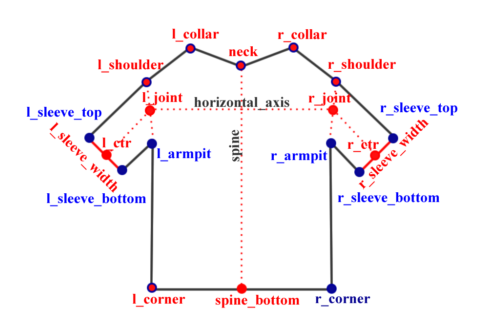
\includegraphics[width=\textwidth]
    	{figures/SOTA_Miller_2011.png}
    \end{subfigure}
    ~
    \begin{subfigure}[r]{0.49\textwidth}
	   \centering
		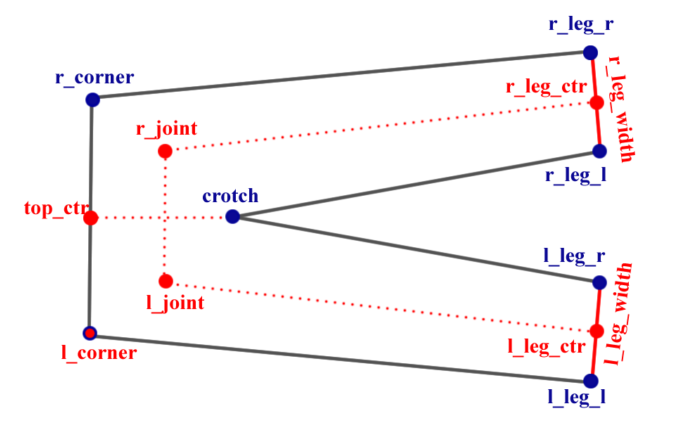
\includegraphics[width=\textwidth]
		{figures/SOTA_Miller_2011-2.png}
	\end{subfigure} 
   	\caption[dummy]{Models proposed by Miller in \cite{Miller2011} \comment{(?)}. The points shown in red are the skeletal points selected to fit the model to the garment data obtained by the vision system. Using those points and the parameters represented by the red segments the rest of the key points and dimensions are calculated to complete the model.}
   	\label{fig:SOTA_Miller_2011}
\end{figure}

A method for classifying and estimating the poses of deformable objects is presented in \cite{Li2014ICRA}. This method consists in creating a training set of deformable objects by off-line simulation of different garments, extracting depth images from different points of view. Then, a codebook is built for a set of different poses of each deformable object by extracting features from the dataset and applying sparse coding and dictionary learning. With this codebook, classifying deformable objects on different categories and estimating their current pose is possible, for later regrasping or folding the garment.

The previous method was improved in \cite{Li2014IROS}, by extracting the features directly from the 3D data, dividing the hanging garment in different cells via layers, rings and sectors of the bounding cylinder. Each of the sectors becomes a binary feature, using the Signed Distance Function to check if the cell is inside the voxel where the center of the cell belongs, and is then arranged in a feature vector. A Hamming distance, whose weights are learned from the simulated dataset merged with some models reconstructed from real word Kinect point clouds, is used to estimate the object category and pose given an input reconstructed mesh model.

\begin{figure}[thpb]
    \centering
    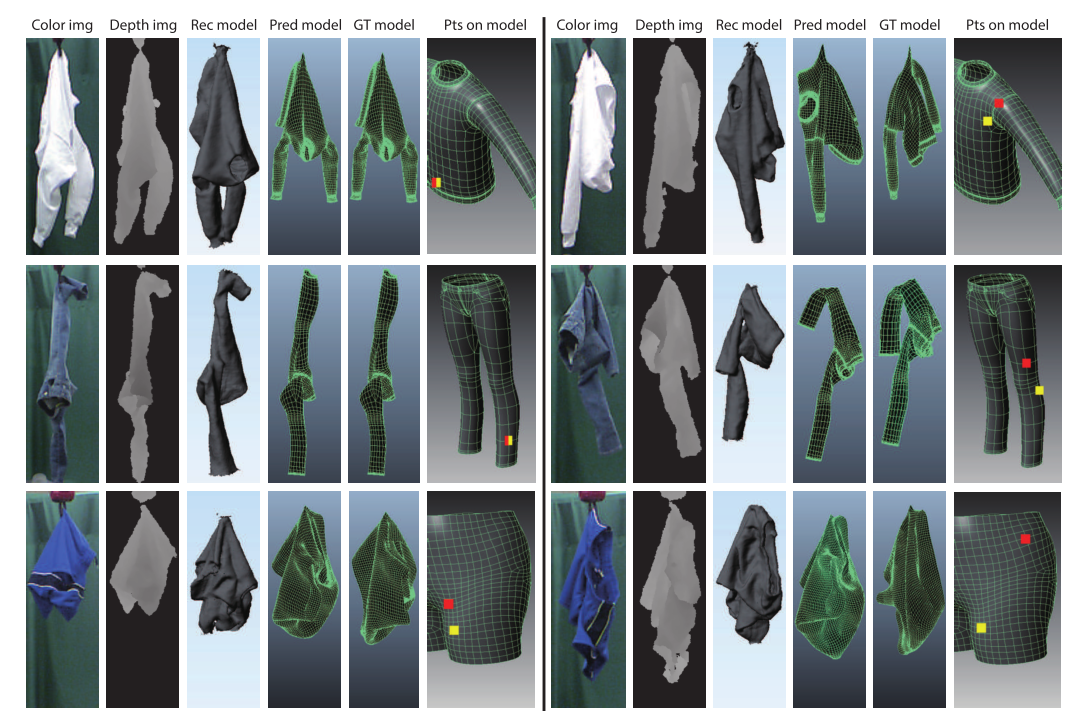
\includegraphics[width=\textwidth]{figures/SOTA_Li_2014-2.png}
    \caption[dummy]{Sample result from experiments carried out by Li in \cite{Li2014IROS} \comment{(?)}. Each row corresponds to a different garment, grouped into 2 different views of each garment (columns 1-6 and 7-12). The first and second pictures of each group correspond to color and depth images captured with the Kinect sensor. Third picture shows the reconstucted model for each garment. The remaining pictures show, from left to right, the predicted simulated model, the ground truth simulated model and the predicted and ground truth grasping points, overlaid over a 3D view of the unfolded garment.
    }
    \label{fig:SOTA_Li_2014}
\end{figure}

\section{Garment Manipulation-Based Approaches}
\label{sota:garment_manipulation_based}
Clothing article manipulation is another field in which extensive work has been done. Based on the previous recognition algorithm, Li presents in \cite{Li2015ICRA} a method for unfolding deformable objects with a bi-manipulator robot. With this method, the robot is capable of taking a clothing article from an unknown state to a known state by iterative regrasping, detecting the most suitable grasping points in each state to achieve its goal. For locating the most suitable grasping points, the 3D point cloud obtained by the robot is matched to the mesh model, that incorporates the information about the best regions to grasp in order to unfold the garment.

\begin{figure}[thpb]
    \centering
    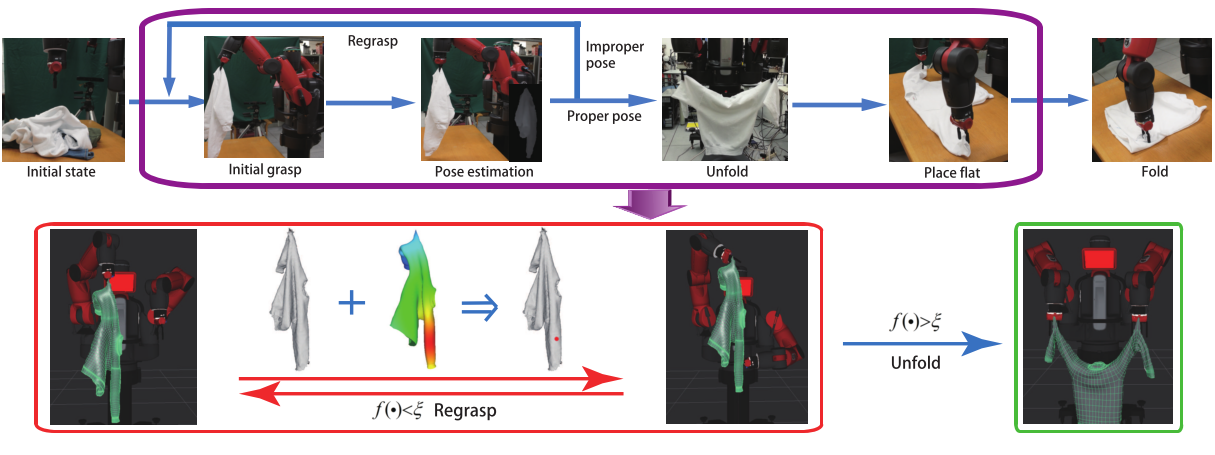
\includegraphics[width=\textwidth]{figures/SOTA_Li_2015.png}
    \caption[dummy]{The complete pipeline of dexterous manipulation of deformable objects presented by Li in \cite{Li2015ICRA} \comment{(?)}. The pipeline of a robot folding a garment from a random state spans initial grasping, pose estimation, regrasping and placing the garment on a table. Actions indicated in the red rectangle, regrasp the object and repeat the pose estimation step, will be performed by the the robot in case that the recognition is not successful.}
    \label{fig:SOTA_Li_2015}
\end{figure}

The method introduced by Cusumano-Towner et al. in \cite{Cusumano-Towner2011} allows a bi-manipulator robot to identify a clothing article, estimate its current state and achieve a desired configuration, generalizing to previously unseen garments. For that purpose, the robot uses a Hidden Markov Model (HMM) throughout a sequence of manipulations and observations, in conjunction with a relaxation of a strain-limiting finite element model for cloth simulation that can be solved via convex optimization.

\begin{figure}[thpb]
    \centering
    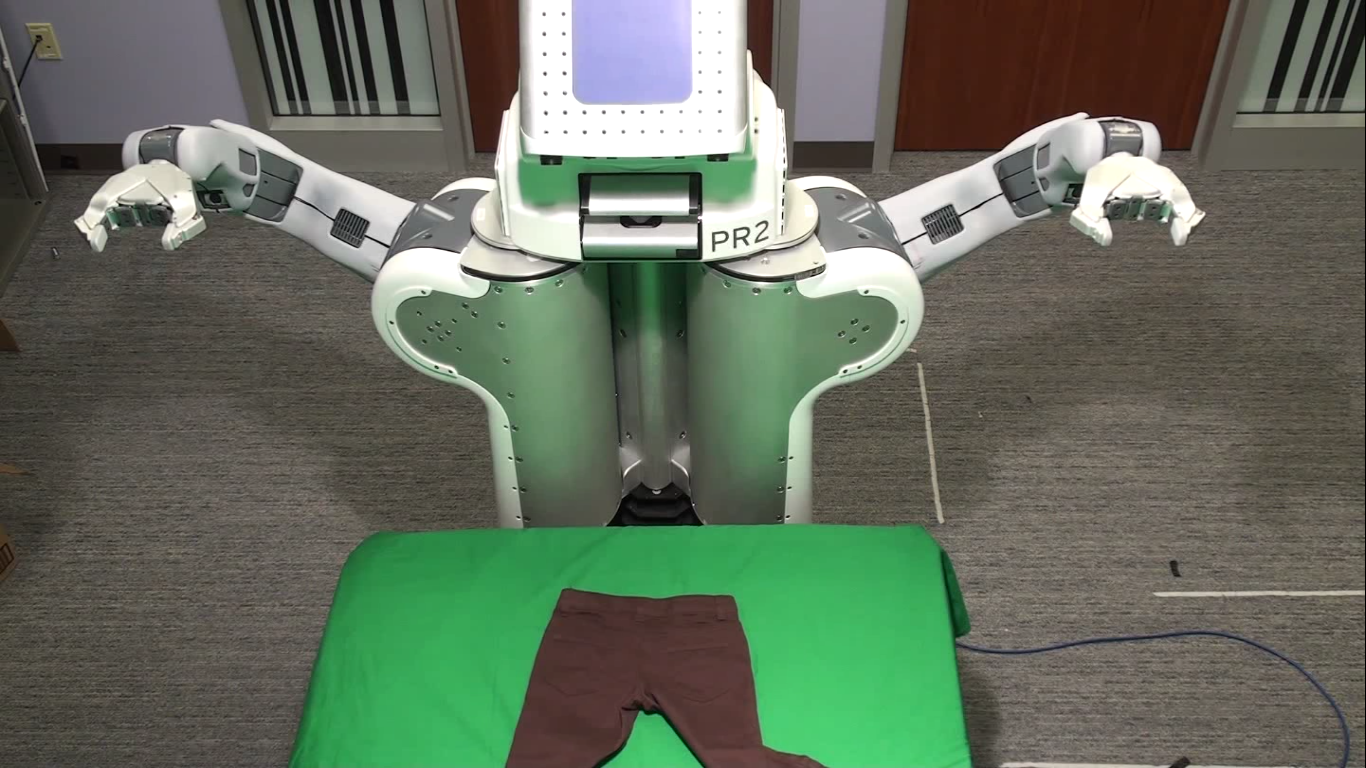
\includegraphics[width=\textwidth]{figures/SOTA_Cusumano_PR2.png}
    \caption{PR2 robot during the manipulation of a pair of pants in order to reconfigure their pose. \comment{add stuff here}}
    \label{fig:SOTA_Cusumano_2011}
\end{figure}

Osawa et al. propose in \cite{Osawa2006} a method to unfold garments in order to classify them. It consists in alternatively regrasping clothing and expanding them using a two-arms manipulator. The garment is grasped with one arm and the lowest point is located by rotating the piece of clothing, which is used as a grasping point for the other arm. If the garment has any fold when extended, it is placed over a flat surface to repeat this process util the the garment is fully spread out.

To detect the best grasping points for a clothing article, Ramisa \cite{Ramisa2012} performs the identification in a single step, even with highly wrinkled clothes. This detector is based in a Bag of Features detector, using as input a combination of appearance and 3D geometric features.

The most similar work we can find in the related literature is the method for unfolding clothes presented by Willimon et al. in \cite{Willimon2011}. Their method, which also focuses in clothes unfolding prior to automated folding, use several features obtained from a depth image, such as peak regions and corners location, to determine the location and orientation most suitable for interaction with the garment. Two main steps are performed: first, the clothing article is flattened using RGB information from the camera and, then, depth information is used to extract the features used to estimate how to unfold the garment.

\section{CloPeMa European Project}
\label{sota:clopema}

CloPeMa\footnote{\url{http://www.clopema.eu/}} is a recent EU-FP7 research project (2012-2015) whose objective is to advance the state of the art in perception and manipulation of fabric, textiles and garments. The project's official logo can be seen in Figure \ref{fig:SOTA_CloPeMa_logo}.

\begin{figure}[thpb]
    \centering
    
\includegraphics[width=0.7
    \textwidth]{figures/SOTA_CloPeMa_logo.png}
    \caption{CloPeMa European Project logo.}
    \label{fig:SOTA_CloPeMa_logo}
\end{figure}

 As part of the CloPeMa project, a method to detect single folds has been presented by Mariolis et al. in \cite{Mariolis2013, Mariolis2015}. In order to detect such folds, a database of unfolded clothes templates is built in the first place. These templates are later used to perform a shape matching between the folded garment shape, obtained by the camera, and the unfolded garment model. This process is iterative, and the initial results are feedbacked to adapt the model for a better fit. 

\begin{figure}[thpb]
    \centering
    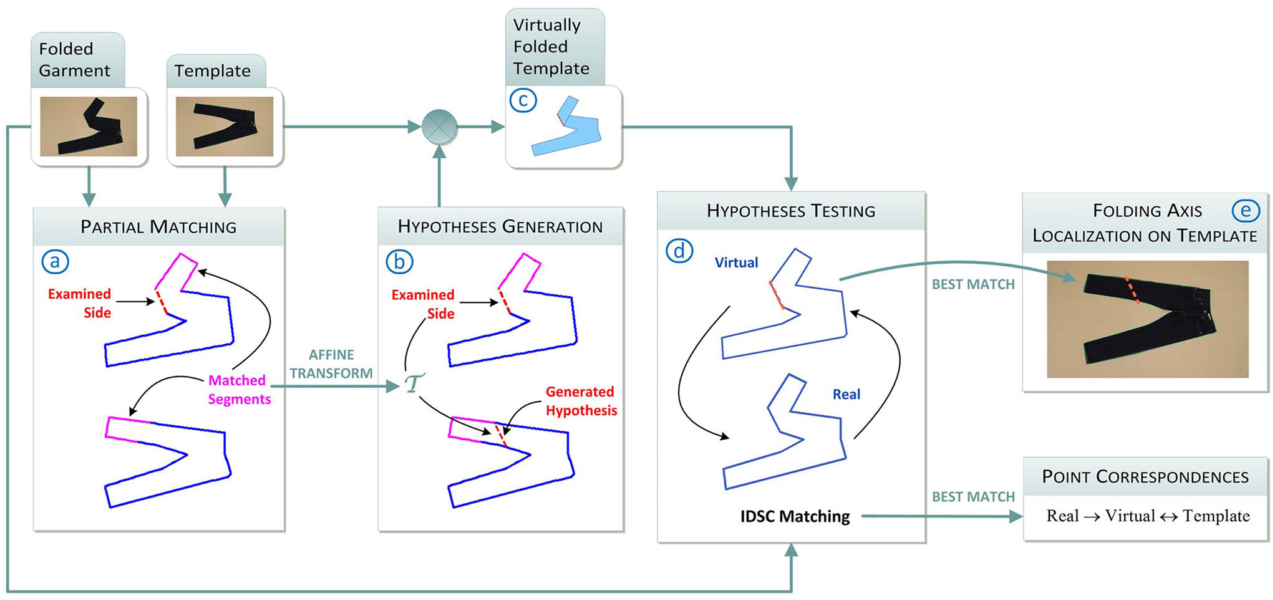
\includegraphics[width=\textwidth]{figures/SOTA_Mariolis_2015.png}
    \caption[dummy]{Block diagram of the method proposed by Mariolis in \cite{Mariolis2015}. This method performs shape matching of folded garments and unfolded templates. In the first stages the garment and the unfolded template are matched and transformed to generate an hypothesis. An Inner Distance Shape Contexts (IDSC) algorithm is then applied to test the hypotheses and find the best match for the folding axis on the template.}
    \label{fig:SOTA_Mariolis_2015}
\end{figure}

Stria et al. propose in \cite{Stria2014, Stria2014IROS} a polygon-based model for clothes configuration recognition using the estimated position of the most important landmarks in the clothing article. Once identified, these landmarks can be used for automated folding using a robotic manipulator. The clothes contour is extracted from a RGB image and processed using a modified grabcut algorithm and dynamic programming methods are used to fit it to the polygonal model.

\begin{figure}[thpb]
    \centering
    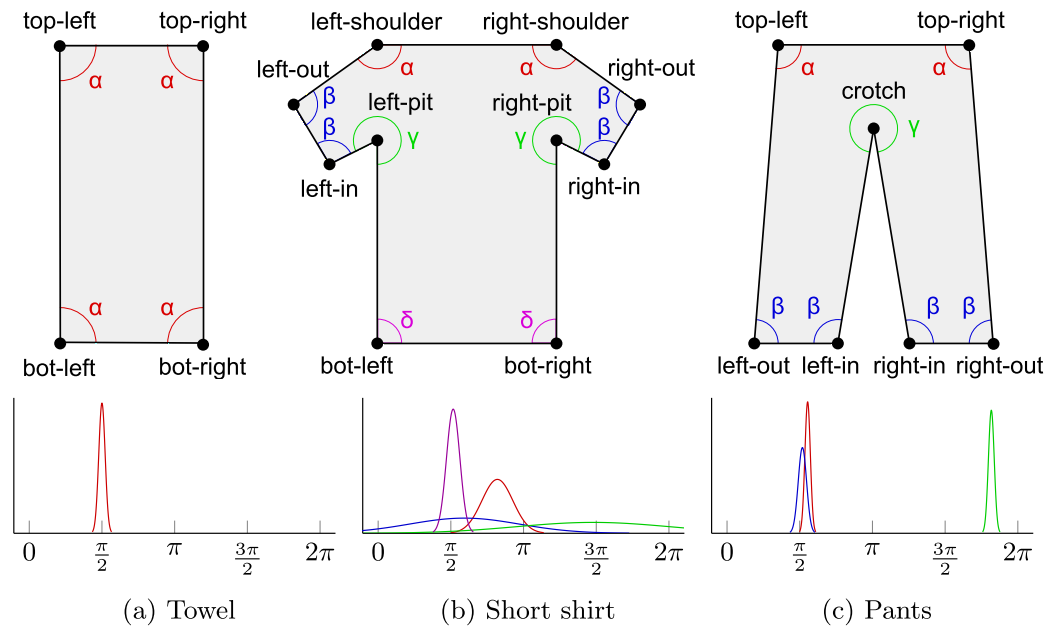
\includegraphics[width=\textwidth]{figures/SOTA_Stria_2014-3.png}
    \caption[dummy]{Polygonal models proposed by Stria et al. in \cite{Stria2014} for several categories of clothes. The upper figures show the different angular parameters that comprise the model of each garment category. Beneath each one of them, the circular distribution of each of the angles of the model occurring in real garments.}
    \label{fig:SOTA_Stria_2014}
\end{figure}


Doumanoglou et al. follow in \cite{Doumanoglou2014ECCV} an approach based on Active Random Forests to recognize clothing articles from depth images. This classifier allows the robot to perform actions to collect extra information in order to disambiguate the current hypotheses, such as changing the viewpoint. In \cite{Doumanoglou2014ICRA} they extend this approach to detect the optimal grasping points to unfold the garment.


\begin{figure}[thpb]
    \centering
    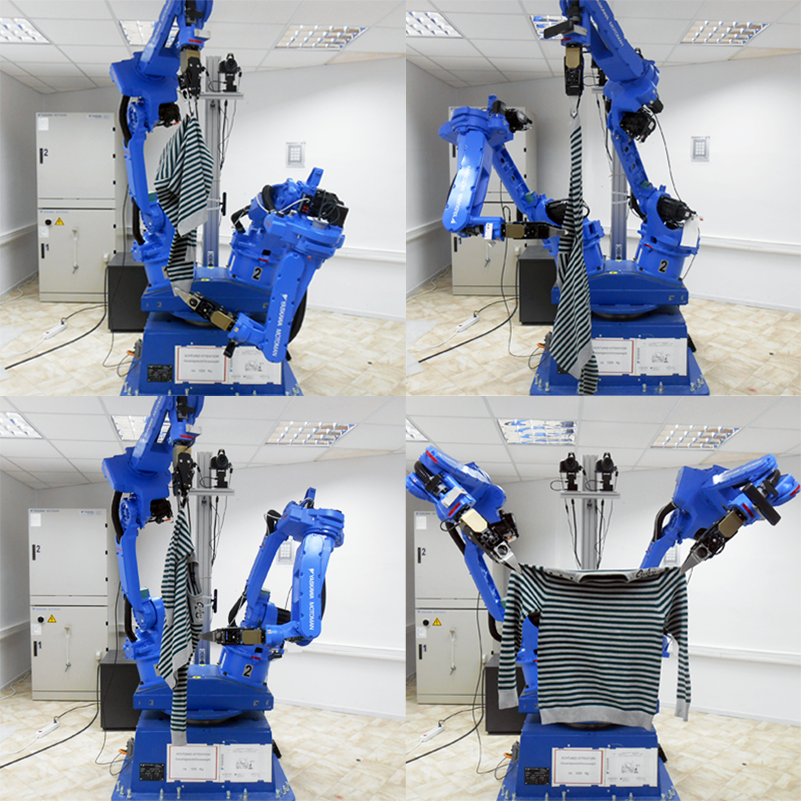
\includegraphics[width=0.95
    \textwidth]{figures/SOTA_Doumanoglou_2014.png}
    \caption[dummy]{CloPeMa's bimanipulator robot manipulating a garment using the approach presented by Doumanoglou et al. in \cite{Doumanoglou2014ECCV}. The robot is made of two industrial robotic MA1400 arms, used in the welding industry, and has a binocular system composed of two Nikon DSLR cameras (D5100). Other sensors, such as force or photometric close-rande sensors are also integrated in the robot. The robot is using Active Rando Forests to perform garment recognition, changing the garment pose if disambiguation is required.}
    \label{fig:SOTA_Doumanoglou_2014}
\end{figure}


%Some work on wrinkles removal has been made by Sun et al. \cite{Sun2015} with a stereo vision system and a dual manipulator robot. Wrinkles are first identified  using a depth map of the cloth, which is later B-spline smoothed and parsed by shape and topology into different wrikle structures, that are later ranked by size and removed.
